\makeatletter

\long\gdef\versochapter#1{
  \vspace*{3cm}
  \minipage{\textwidth}
  \hfill\includegraphics[width=0.5\textwidth]{\chapterimage@cx}\par
  \vspace*{6pt}
  \hfill\minipage{0.75\textwidth}
  {\HUGE\bfseries\flushright #1\endflushright}
  \endminipage
  \endminipage
  \newpage


\vspace*{10cm}
\@specialfalse
\@openleftfalse
\@openanyfalse
\@openrighttrue
}


\newgeometry{bottom=2.5cm}

\cxset{
   chapter image/.code={\def\chapterimage@cx{#1}},
   chapter opening/.is choice,
   chapter opening/verso/.code={\@specialtrue\@openlefttrue
   \gdef\customdesign@cx##1{\versochapter{##1}}}
}

\cxset{
 custom=versochapter,
 chapter image={./images/vespa.jpg},
 chapter opening=verso,
 name={},
 numbering=none,
 number font-size=LARGE,
 number font-family=rmfamily,
 number font-weight=bfseries,
 number before=,
 number dot={},
 number after=,
 number position=leftname,
 chapter font-family=sffamily,
 chapter font-weight=\normalfont,
 chapter font-size=\Large,
 chapter before={\vspace*{0pt}\par},
 chapter after={\hfill\hfill\par},
 chapter color={black!90},
 number color=purple,
 title beforeskip={\vspace*{0pt}},
 title afterskip={\vspace*{0.4\textheight}\par},
 title before={},
 title after={},
 title font-family=sffamily,
 title font-color=purple,
 title font-weight=bfseries,
 title font-size=LARGE,
 header style=plain,
 pagestyle=plain,
 authorblock=false,
}

\makeatletter
\@specialtrue
\makeatother



\chapter{Verso Chapters}

\parindent1.5em
{\HUGE V}erso chapter openings are not common. One design that I found quite attractive is \lipsum[1-3] \textit{From Western attitudes toward death from the middle ages to the present}, Philippe Ari\'es. London, 1974.

\begin{figure}
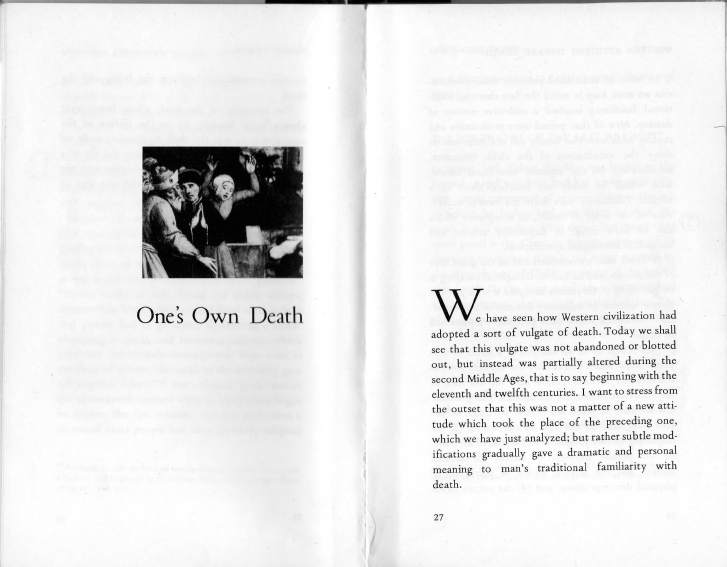
\includegraphics[width=\textwidth]{./chapters/versochapter01.png}
\caption{Chapter opening on verso page.}
\end{figure}

\makeatletter
\@specialfalse
\makeatother
